\section{Project analysis and System requirements}
\phantomsection

\subsection{Problem Definition}
The platform OpenMedia is a rather complex system consisting from several parts. That is why is crucial to break it into smaller modules and logical components that can communicate with each other. There are lots of parts which the application should consist of: data fetching, cleaning the articles and enriching them with proper metada, interactive modern web application, efficiently storing the data, running tasks independently, communication between system components, how to implement asynchronous messaging between modules, smart visualization of the data, what are the dependencies of some specific technologies, how this dependencies will co-work in combination with the rest of the system. If looked from a bigger scale the problem is not that simple, that's why a deeper level of structured granularity is required.

\subsection{Project Analysis}
The project OpenMedia is a platform used to provide visual models and statistic result based on online media sources from Republic of Moldova. It aims to collect the available articles found on the public sources and use them as a generic source for extracting useful results to be provided to visualization tools. The features offered by OpenMedia will be tools for querying for the desired keywords, in order to construct frequency plots, with options to see to what sources it belongs to. Also it will bring trend detection utilities. By selecting a range of time, it will render the most mentioned terms, and construct bar charts thus communicating the relevance of the popularity.

The platform will consist from two major parts.
\begin{itemize}
    \item Data gathering platform
    \begin{itemize}
        \item Fetching the article pages
        \item Extracting the article
        \item Storing the article
        \item Enriching with textual metadata
    \end{itemize}
    \item Web Client platform
    \begin{itemize}
        \item A simple and intuitive design
        \item Launching asynchronous tasks
        \item Receiving the finished
        \item Visualization of results
    \end{itemize}
\end{itemize}

\subsubsection{Data gathering platform}
This part of the application is focused on gathering data, cleaning and baking it. Simply put, all the heavy lifting of textual data preprocessing is done by this part of the platform. In the figure \ref{data_gathering_mock} is mocked the activity layers of the application. It is important to deliver the data in a format easily operable by the application because the amount of data analysis tricks becomes more various. To be more specific, it is up to client platform to choose the techniques of data consumption. On the one hand it does not sound as an optimized solution but on the other hand it offers flexibility. Data collection is a long and tedious process, that is why it should be better run once. More than that it is advised that all the data changes should be managed in a separate copy. Keeping each stage of data in an immutable state is a wise move. Redundancy is a better choice due to the fact that a project is prone to changes. Running the entire gathering operation from the bottom just in order to add a new feature sounds lethal to a business solution. That is why the OpenMedia platform saves each stage of data.

The articles used by the platform are the public sources of the online media of Republic of Moldova. These are Unimedia, Timpul and Publika. As a future goal is intended to include the other available resources, in order to make the platform more media agnostic. Adding to the system as many resources as possible is a key part of OpenMedia philosophy. The idea is that media sources are usually biased usually by political reasons, meaning that a research in a political area could lead to a less viable result. Beyond that the platform would provide means to deduce predispositions to some governmental parties.



\begin{figure}[!ht]
\centering
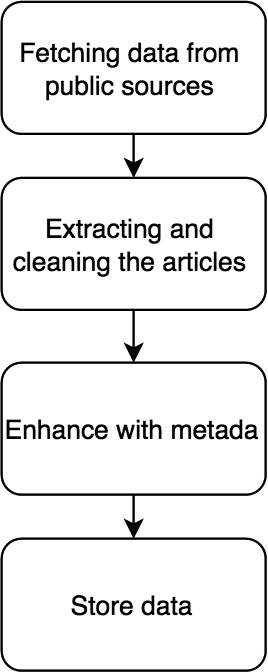
\includegraphics[width=3.8cm]{1_data_gathering}
\caption{Data Gathering platform mockup}\label{data_gathering_mock}
\end{figure}

\subsubsection{Web Client platform}
The client side will represent a web application, a minimalistic layer used for communication between user and the platform. Having a web infrastructure offers the opportunity to make the application easy to access. The only requirement being a modern web browser like Google Chrome, Firefox etc. The focus of the application is to make available the following functionalities.
\begin{itemize}
    \item execute queries on specified words
    \item execute trend detection queries on specified date rang
    \item display frequency line charts
    \item display trends popularity bar charts
\end{itemize}

This are the basic functionalities provided by the client application. Of course here are also included details such as specifying the media resource, in order to be able to compare the results and extract some useful conclusions from it. The goal is to make the user experience as natural as possible. And due to the fact that he number of functionalities are not so various, creating a natural flow of events will not represent an essential problem. But it should be taken into consideration that a reduced amount of functionalities does not mean a reduced amount of operations. The whole sequence of events is rather complex. It will be described step by step in the next pages of the report.

\begin{figure}[!ht]
\centering
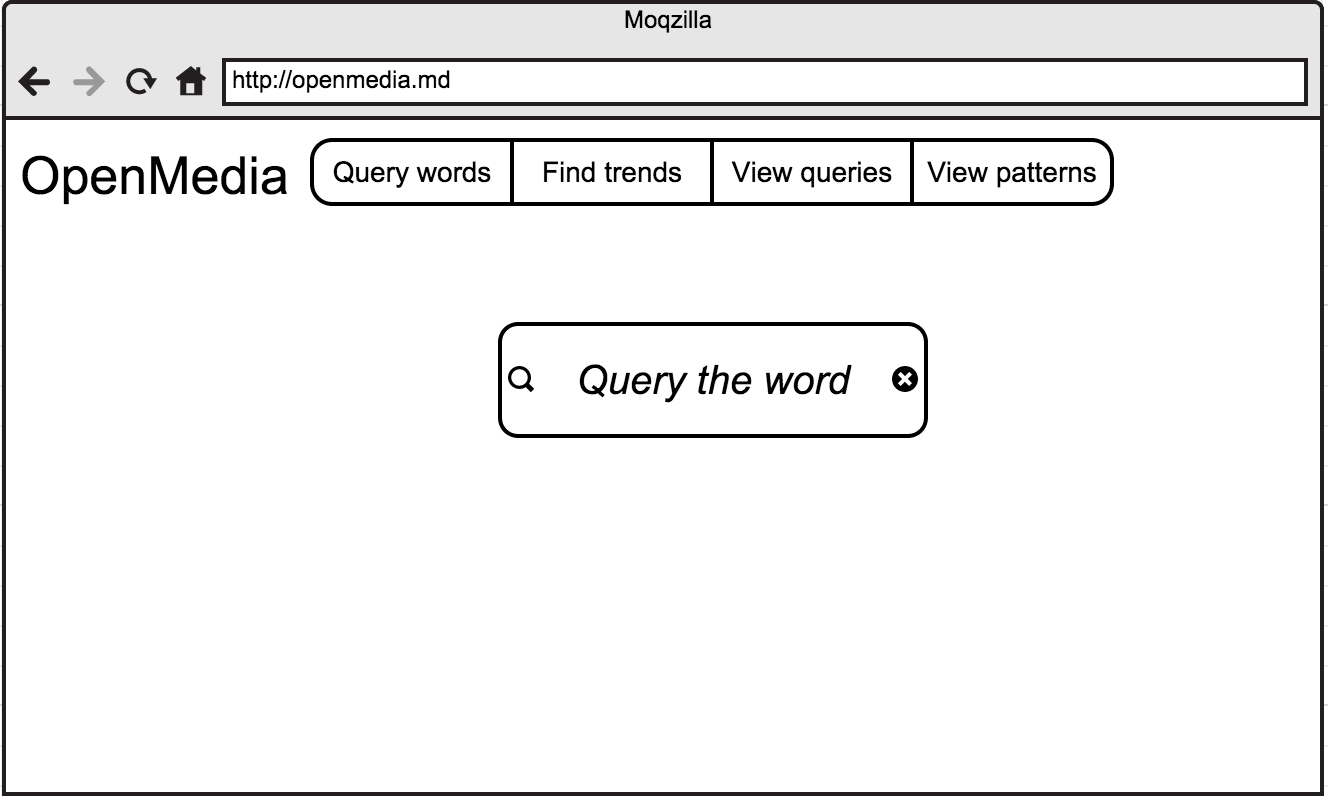
\includegraphics[width=13cm]{1_app_mock_1}
\caption{Primary page view}\label{app_mock_1}
\end{figure}

In order to make an expected view of the application. There are presented some mockups of the web applications. In figure \ref{app_mock_1} is represented the main page. The user has the input box used to execute queries related to word frequency. Because the query execution latency is going to be pretty long, the application is intended to work in an asynchronous way. So after the clicking, a notification will pop up informing that a query was started. Also a pop up notification will be displayed when there are news about the result. After which the result can accessed by clicking on View Queries button. By selecting the specific word, application is transitioning to a result view. The mockup of the page can be observed in figure \ref{1_app_mock_2}. A  plot is rendered representing the intensity per month which the word was mentioned. According to date range, the necessary conclusions be drawn. For example when was the specific word at it's peak. When it started to become less popular, what are the spikes, what caused the spikes. This might prove quite valuable information if examined from the right angle. The good part that anyone interested of statistic results can use it. Starting from business entrepreneurs which are trying to research the trendiness of a specific product, a journalist which is interested in popularity of a specific event or entity. The great part about it is that a personal set of queries can be done, thus building a custom aggregation of analytical results

\begin{figure}[!ht]
\centering
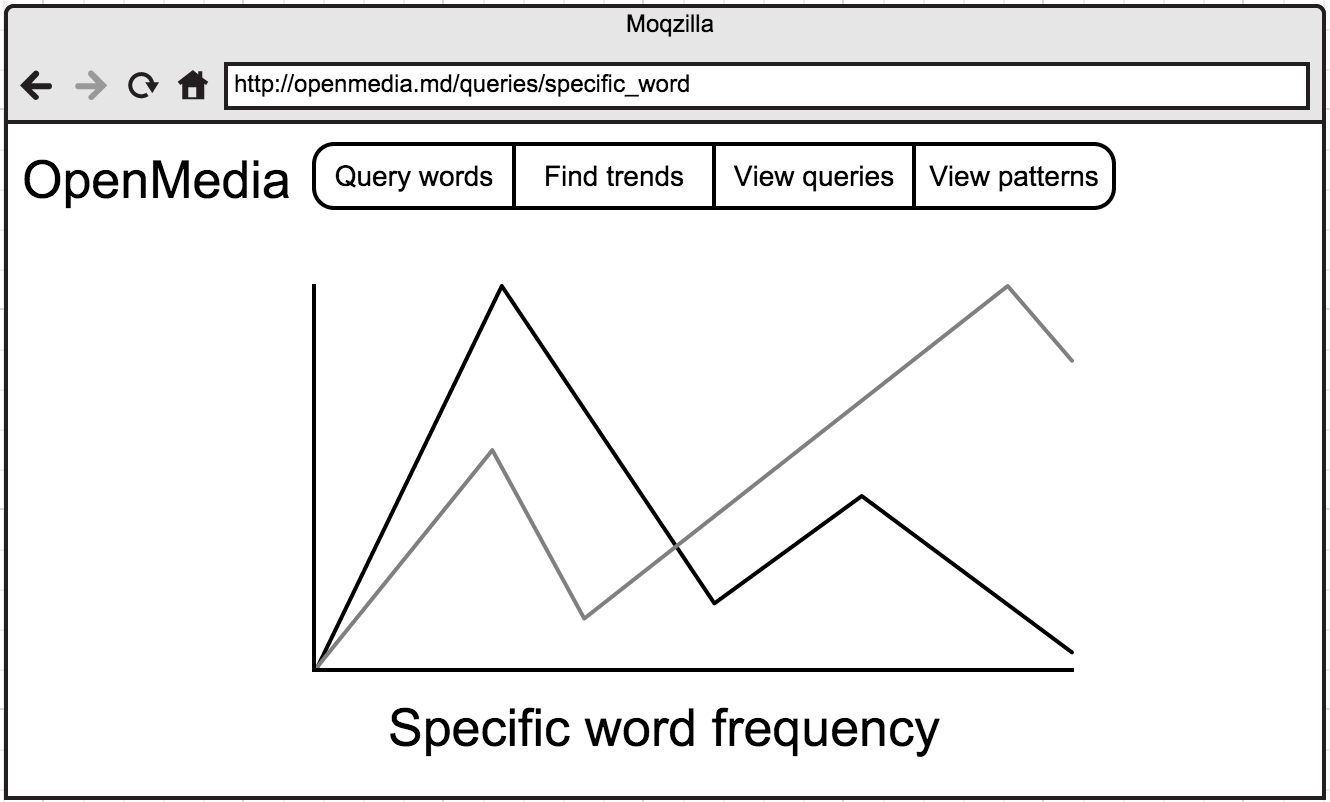
\includegraphics[width=13cm]{1_app_mock_2}
\caption{Frequency plot view}\label{app_mock_2}
\end{figure}

\subsection{Theoretical analysis}
Considering the complexity of the platform, a right amount of research is required in order to construct a workable product. The project OpenMedia consists of two independent separate product. Because both make part of the same new evolving field, data science, the final product represents a usable product which can be used on a local scale. Now will follow a more detailed description of various aspects of the platform, regarding the technologies best suited for building the application, the concepts involved under the hood, means of solving some specific problems.

\subsubsection{Data Mining}
According to wikipedia sources, data mining, an interdisciplinary subfield of computer science, is the computational process of discovering patterns in large data sets involving methods at the intersection of artificial intelligence, machine learning, statistics, and database systems. The overall goal of the data mining process is to extract information from a data set and transform it into an understandable structure for further use. \cite{wiki_data_mining}

\begin{figure}[!ht]
\centering
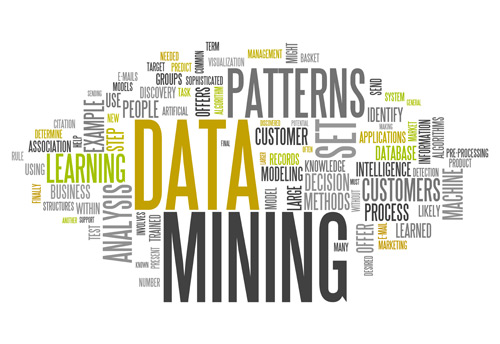
\includegraphics[width=9cm]{1_data_mining}
\caption{Data Mining}\label{data_mining}
\end{figure}

The actual data mining task is the automatic or semi-automatic analysis of large quantities of data to extract previously unknown interesting patterns such as groups of data records (cluster analysis), unusual records (anomaly detection) and dependencies (association rule mining). This usually involves using database techniques such as spatial indices. These patterns can then be seen as a kind of summary of the input data, and may be used in further analysis or, for example, in machine learning and predictive analytics. For example, the data mining step might identify multiple groups in the data, which can then be used to obtain more accurate prediction results by a decision support system. Neither the data collection, data preparation, nor result interpretation and reporting are part of the data mining step, but do belong to the overall KDD process as additional steps.

The related terms data dredging, data fishing, and data snooping refer to the use of data mining methods to sample parts of a larger population data set that are (or may be) too small for reliable statistical inferences to be made about the validity of any patterns discovered. These methods can, however, be used in creating new hypotheses to test against the larger data populations

\subsubsection{Text processing}
The aim of text processing is to consume unstructured textual information, extract important numeric indices and make it accessible for various data mining, statistical algorithms. Information can be extracted to derive summaries for the words contained in the documents or to compute summaries for the documents based on the words contained in them. Hence a text analysis can be performed on clusters of words used in documents. Another approach could be to analyze documents and determine similarities between them or how they are related to other variables of interest. In a nutshell, text processing is an action of transforming text into numbers, and other metadata, eventually used in predictive data mining projects, machine learning, data warehousing, etc.

Unstructured text is very common, and in fact may represent the majority of information available to a particular research or data mining project. A relevant example of textual data analysis application would be automatic filtering of undesirable junk emails based on certain terms and words that are most likely to be met. In such manner the obnoxious mails can be discarded. It can be taken even further, such kind of applications could be used in a bigger systems for routing messages, based on email contents, to the appropriate department. Or sent back to sender, in case of detecting some obscure content, with a request to change the body.

A powerful use case could be to process the contents of a particular Web portal. For example for extracting relevant specific block, and determining the most frequently mention word, thus deriving the most important terms of the web application. It's easy to observe how this kind analysis could deliver valuable business intelligence. This kind of use case resembles very much with system requirements of the OpenMedia platform. Given that the aim is to crawl all the possible articles of the media portals, and perform data mining algorithms on it. And as a result to have a set of services providing statistical .

Another curious aspect of data processing is that there are two angles of processing textual documents. First is many data to few documents, and second is small data from lots of documents. For instance, on case is performing complex text analysis tasks on few lengthy resources (like books) and the another is extracting key values concepts from tweeter messages which have a limit size of 140 characters. The second case is more compliant to statistic algorithms by the fact that the amount of data sources is much bigger. This means that OpenMedia is a perfect playground for applying various statistic models.

One think that should be taken into consideration is the data indexing. Indexing is a feature usually provided by the modern databases. The idea behind it is to create additional data, resembling a hash map data structure, which allows to search data much faster by a specific field. For instance we have classic SQL database with a "user" schema which has "name" field. If the system using the database is frequently searching for "user" entity by it's "name" then it is the most wise to perform indexing on the table. This will add additional data on the disk, instead the search queries by "name" would be much faster. The point is when dealing with big chunks of textual data indexing by each word my not prove a sensible option. Instead some tricks can be applied, like removing certain characters, words bounded by some length, frequently used stop words like "the", "a", "of" etc. Another idea would be a custom indexing task which would detect synonyms and index as the same entity when a pair is found. One more thing would be to remove the rarely used words which do not offer much information about the text.

\subsubsection{Data storage}

\subsubsection{Semantic analysis}
Stemming algorithms. An important pre-processing step before indexing of input documents begins is the stemming of words. The term "stemming" refers to the reduction of words to their roots so that, for example, different grammatical forms or declinations of verbs are identified and indexed (counted) as the same word. For example, stemming will ensure that both "traveling" and "traveled" will be recognized by the text mining program as the same word.

Support for different languages. Stemming, synonyms, the letters that are permitted in words, etc. are highly language dependent operations. Therefore, support for different languages is important.
\subsubsection{Map reduce}
\subsubsection{Hadoop}
\subsubsection{REST and SOAP services}
\subsubsection{Modern web application}
\subsubsection{Web Sockets}
\subsubsection{Data Visualization}
\subsubsection{Web Crawling}

A web crawler (also known as a robot or a spider) is a system for the
bulk downloading of web pages. Web crawlers are used for a variety of
purposes. Most prominently, they are one of the main components of
web search engines, systems that assemble a corpus of web pages, index
them, and allow users to issue queries against the index and find the web
pages that match the queries. A related use is web archiving (a service
provided by e.g., the Internet archive [77]), where large sets of web pages
are periodically collected and archived for posterity. A third use is web
data mining, where web pages are analyzed for statistical properties,
or where data analytics is performed on them (an example would be
Attributor [7], a company that monitors the web for copyright and
trademark infringements). Finally, web monitoring services allow their
clients to submit standing queries, or triggers, and they continuously
crawl the web and notify clients of pages that match those queries (an
example would be GigaAlert [64]).

Web crawling is the process of gathering pages from Web, in
order to index them and support a search engine. The objective of crawling
is to quickly and efficiently gather as many useful web pages as possible,
together with the link structure that interconnects them.

Crawling is performed by anywhere from one to potentially hundreds of
threads, each of which loops through the logical cycle in Figure 20.1. These
threads may be run in a single process, or be partitioned amongst multiple
processes running at different nodes of a distributed system. We begin by
assuming that the URL frontier is in place and non-empty and defer our description
of the implementation of the URL frontier to Section 20.2.3. We
follow the progress of a single URL through the cycle of being fetched, passing
through various checks and filters, then finally (for continuous crawling)
being returned to the URL frontier.
A crawler thread begins by taking a URL from the frontier and fetching
the web page at that URL, generally using the http protocol. The fetched
page is then written into a temporary store, where a number of operations
are performed on it. Next, the page is parsed and the text as well as the
links in it are extracted. The text (with any tag information – e.g., terms in
boldface) is passed on to the indexer. Link information including anchor text
is also passed on to the indexer for use in ranking in ways that are described
in Chapter 21. In addition, each extracted link goes through a series of tests
to determine whether the link should be added to the URL frontier.
First, the thread tests whether a web page with the same content has already
been seen at another URL. The simplest implementation for this would
use a simple fingerprint such as a checksum (placed in a store labeled "Doc
FP’s" in Figure 20.1). A more sophisticated test would use shingles instead
of fingerprints, as described in Chapter 19.
Next, a URL filter is used to determine whether the extracted URL should
be excluded from the frontier based on one of several tests. For instance, the
crawl may seek to exclude certain domains (say, all .com URLs) – in this case
the test would simply filter out the URL if it were from the .com domain.
A similar test could be inclusive rather than exclusive. Many hosts on the
Web place certain portions of their websites off-limits to crawling, under a
ROBOTS EXCLUSION standard known as the Robots Exclusion Protocol. This is done by placing a
PROTOCOL file with the name robots.txt at the root of the URL hierarchy at the site. Here
is an example robots.txt file that specifies that no robot should visit any URL
whose position in the file hierarchy starts with /yoursite/temp/, except for the
robot called “searchengine”.

The robots.txt file must be fetched from a website in order to test whether
the URL under consideration passes the robot restrictions, and can therefore
be added to the URL frontier. Rather than fetch it afresh for testing on
each URL to be added to the frontier, a cache can be used to obtain a recently
fetched copy of the file for the host. This is especially important since
many of the links extracted from a page fall within the host from which the
page was fetched and therefore can be tested against the host’s robots.txt
file. Thus, by performing the filtering during the link extraction process, we
would have especially high locality in the stream of hosts that we need to test
for robots.txt files, leading to high cache hit rates. Unfortunately, this runs
afoul of webmasters’ politeness expectations. A URL (particularly one referring
to a low-quality or rarely changing document) may be in the frontier for
days or even weeks. If we were to perform the robots filtering before adding
such a URL to the frontier, its robots.txt file could have changed by the time
the URL is dequeued from the frontier and fetched. We must consequently
perform robots-filtering immediately before attempting to fetch a web page.
As it turns out, maintaining a cache of robots.txt files is still highly effective;
there is sufficient locality even in the stream of URLs dequeued from the URL
frontier.
URL NORMALIZATION Next, a URL should be normalized in the following sense: often the HTML
encoding of a link from a web page p indicates the target of that link relative
to the page p. Thus, there is a relative link encoded thus in the HTML of the
page en.wikipedia.org/wiki/Main_Page

Finally, the URL is checked for duplicate elimination: if the URL is already
in the frontier or (in the case of a non-continuous crawl) already crawled,
we do not add it to the frontier. When the URL is added to the frontier, it is
assigned a priority based on which it is eventually removed from the frontier
for fetching. The details of this priority queuing are in Section 20.2.3.
Certain housekeeping tasks are typically performed by a dedicated thread.
This thread is generally quiescent except that it wakes up once every few
seconds to log crawl progress statistics (URLs crawled, frontier size, etc.),
decide whether to terminate the crawl, or (once every few hours of crawling)
checkpoint the crawl. In checkpointing, a snapshot of the crawler’s state (say,
the URL frontier) is committed to disk. In the event of a catastrophic crawler
failure, the crawl is restarted from the most recent checkpoint.

The raison d’ˆetre for web crawlers lies in the fact that the web is
not a centrally managed repository of information, but rather consists
of hundreds of millions of independent web content providers, each one
providing their own services, and many competing with one another.
In other words, the web can be viewed as a federated information repository,
held together by a set of agreed-upon protocols and data formats,
such as the Transmission Control Protocol (TCP), the Domain Name
Service (DNS), the Hypertext Transfer Protocol (HTTP), the Hypertext
Markup Language (HTML) and the robots exclusion protocol. So,
content aggregators (such as search engines or web data miners) have
two choices: They can either adopt a pull model where they will proactively
scour the web for new or updated information, or they could
try to establish a convention and a set of protocols enabling content
providers to push content of interest to the aggregators. Indeed, the
Harvest system [24], one of the earliest search services, adopted such
a push model. However, this approach did not succeed, and virtually
all content aggregators adopted the pull approach, with a few provisos
to allow content providers to exclude all or part of their content
from being crawled (the robots exclusion protocol) and to provide hints
about their content, its importance and its rate of change (the Sitemaps
protocol [110]).
\clearpage